
\begin{figure}[h!]
    \centering
    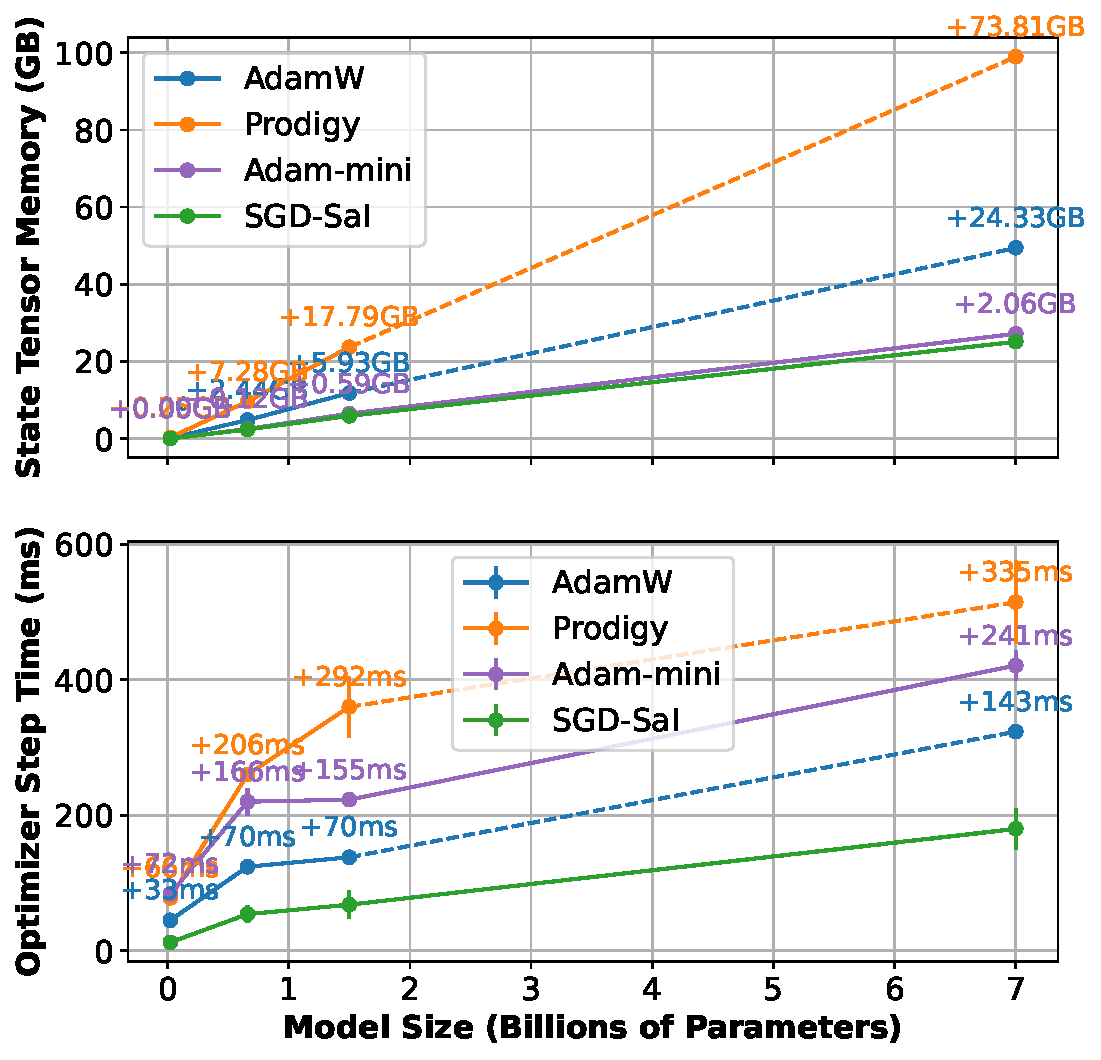
\includegraphics[width=\columnwidth]{images/speed_memory_growth.pdf}
    \caption{The chart illustrates how memory usage and optimizer step time (in wall-clock time) increase with larger model sizes. It highlights the substantial memory overhead of storing optimizer states as model sizes grow. SGD-SaI exhibits significantly lower memory usage than AdamW and has the shortest optimization step runtime. This runtime refers to the wall clock time required for the optimizer step function. All statistics were measured on a single NVIDIA A100-80GB.}
    \label{fig:state_tensor_memory}
\end{figure}

\begin{figure*}
    \centering
    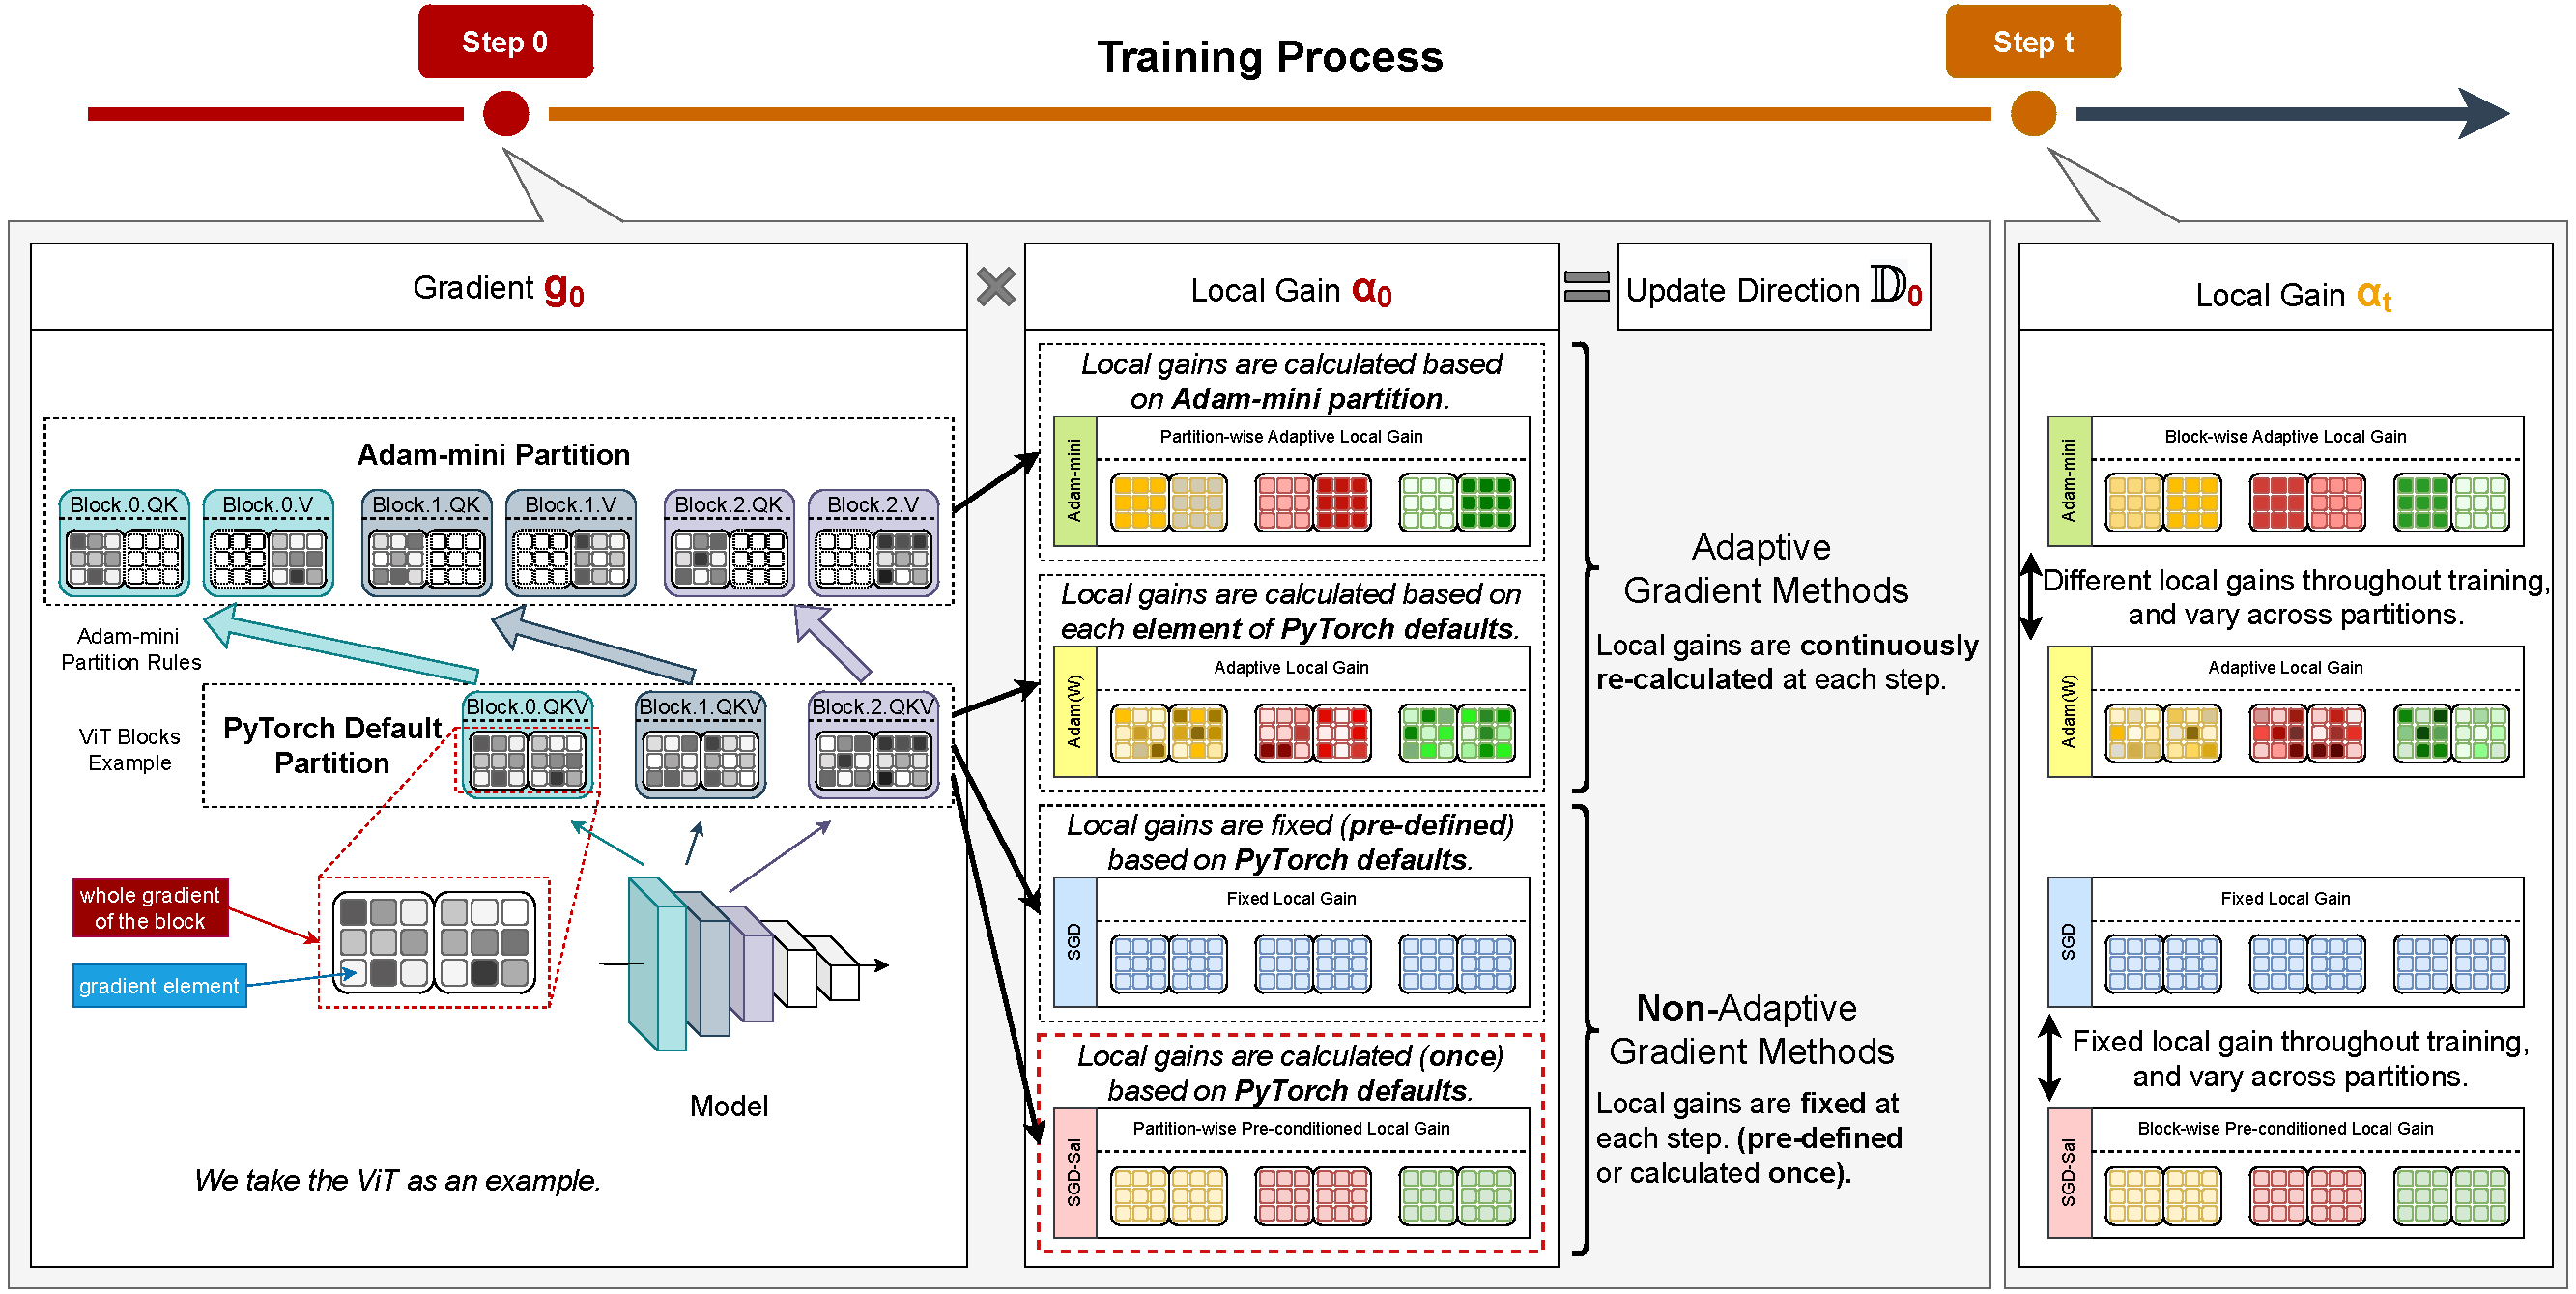
\includegraphics[width=1.\linewidth]{images/algorithm_overview.pdf}
    \caption{This graph illustrates the differences in local gain behaviours exhibited by four optimizers throughout the training process. We present two popular adaptive gradient methods: Adam(W) and the memory-efficient Adam-mini. The local gains for these methods are recalculated continuously at each step based on the gradients. In contrast, SGD and SGD-SaI are both non-adaptive methods, meaning their local gains remain fixed throughout the training.}
    \label{fig:overview}
\end{figure*}



\section{Introduction}
\label{sec:intro}

Stochastic gradient-based optimization methods, such as Stochastic Gradient Descent (SGD), are fundamental to modern machine learning, enabling the successful training of models across a wide range of scientific and engineering applications. However, training objectives and data are often noisy in practice, and gradients may become sparse due to the inherent characteristics of regularization or specific architectural designs. Moreover, architectural differences can introduce imbalances in the learning dynamics across different parameters. To address these challenges, adaptive gradient methods~\cite{cohen2024adaptivegradientmethodsedge} have been developed to handle better non-stationary objectives, noisy data, and sparse gradients. Among these methods, Adam~\cite{kingma2014adam} and AdamW~\cite{loshchilov2019decoupled} have become indispensable for training Transformer-based models, including Large Language Models (LLMs)~\cite{radford2019language, team2023gemini} and Diffusion Models (DMs)~\cite{ho2020denoising, rombach2022highresolutionimagesynthesislatent}. Their popularity stems from their relative robustness and efficiency in optimizing high-dimensional parameter spaces. The core mechanism of Adam's adaptability lies in its second-order momentum term, $v$,  which acts as a local gain~\cite{hinton2012neural}, dynamically adjusting the learning rate for each parameter. This mechanism enables Adam to perform effectively even in noisy or sparse gradients, addressing imbalances in the learning process across different parameters.


However, this adaptability comes with significant costs when the model size scales up. Specifically, Adam requires storing and updating each parameter's first-order (mean) and second-order (variance) momentum terms. This increases memory usage by at least 3x compared to the parameter size alone. For instance, training a 7-billion parameter model in FP32 using Adam requires approximately 50 GB of memory for the state tensors, a significant challenge even with high-end hardware like NVIDIA A100-80G GPUs. Compared to SGD, the memory demand of Adam can be at least double~\cite{zhang2024adamminiusefewerlearning}, posing a severe limitation on the scalability of deep learning research.

Numerous previous works have sought to reduce memory usage by simplifying optimizer states while preserving the adaptive gradient term to address the memory bottleneck while maintaining the effectiveness of adaptive methods. Approaches such as 8-bit Adam~\cite{DBLP:journals/corr/abs-2110-02861}, Adafactor~\cite{shazeer2018adafactor}, and sign-based methods~\cite{bernstein2018signsgdcompressedoptimisationnonconvex, kunstner2023noise} focus on quantizing or sparsifying the optimizer states. Meanwhile, Adam-mini~\cite{zhang2024adamminiusefewerlearning} introduces parameter block grouping to share adaptive learning rates, leveraging Hessian structure insights~\cite{zhang2024transformers} to reduce memory usage. However, these methods often come with trade-offs. Many risk a performance downgrade compared to AdamW. From an efficiency standpoint, these approaches also introduce additional update complexity. Simplified state tensors still require computations based on full gradients for each parameter at each time step, increasing the overall computational burden. Adam-mini, in particular, necessitates fine-grained parameter partitioning~\cite{zhang2024adamminiusefewerlearning}, further complicating its implementation. As a result, these limitations lead to longer optimizer step times, ultimately slowing down the training process.

In this work, we challenge the necessity of adaptive gradient methods for model training and propose a memory- and computation-efficient alternative. We begin by revisiting the foundational motivation behind Adam's use of second-order momentum. Inspired by the concept of the gradient \textbf{Signal-to-Noise Ratio (g-SNR)}~\cite{xiang2023exploiting}, which quantifies the relationship between a gradient's norm and variance, we leverage this metric to analyze and measure gradient distribution differences across parameters. Through empirical analysis, we investigate the temporal consistency for g-SNR during training and explain why this value can be determined at first training iterations. Furthermore, we analysed the g-SNR distribution across different ViT parameters and explored the g-SNR value correlated with varying parameters of type and its architecture characteristics. Building on this, we argue that g-SNR can be leveraged to adjust learning rate scales, balancing the learning progress based on the distribution of gradients. Incorporating a pre-conditioned learning rate scale computed during the first training iteration, called Scaled at Initialization(SaI), facilitates stable training progress without incurring the memory and computational overhead associated with adaptive gradient terms. We call our method \textbf{SGD-SaI}, a novel optimization approach that eliminates the need for adaptive gradient methods, treating them as simple yet effective updates compared to SGD. In summary, our contributions are as follows:

\begin{itemize}
    \item We challenge the necessity of adaptive gradient methods, specifically identified the existing challenges on Adam-like methods and proposed to use constant g-SNR value to replace the second-order momentum to reduce both the memory and computation cost, called \textbf{Scaled at Initialization(SaI)}.
    \item We empirically analysed the statistics of g-SNR on parameters during training and identified its characteristics over time and distribution over parameters. 
    \item We formula our insight into proposed methods, SGD-SaI, solved the long-stand challenge that SGD can not successfully train tasks with transformer architectures and observed outstanding performance in ViT and decoder-only transformer (LLMs).
    \item We extend our empirical analysis to other popular and practical task training, such as LoRA training on LLMs and Diffusion Models(DMs) and traditional CNN tasks. We observed consistent improvement compared to existing SOTA optimizers.
\end{itemize}

